\documentclass[a4paper]{article}
\usepackage[margin=1.5cm]{geometry}

%\documentclass[11pt]{article}
%\usepackage[paperwidth=9cm,paperheight=60cm,margin=0.4cm]{geometry}

\usepackage{multicol}
\usepackage{enumitem}
\usepackage{graphicx}

%Links
\usepackage[colorlinks = true,
            linkcolor = blue,
            urlcolor  = blue,
            citecolor = blue,
            anchorcolor = blue]{hyperref}

%Simbolos matemáticos
\usepackage{amsmath}
\usepackage{amssymb}

%Enumeracion
\usepackage{enumitem}

%Páginas sin numeración
\pagestyle{empty}

%Interlineado
\renewcommand{\baselinestretch}{1.5}

%Arreglar comillas
\usepackage [autostyle]{csquotes}
\MakeOuterQuote{"}

%Macros
\newcommand{\Item}{\item[\stepcounter{enumii}$\blacktriangleright$\textbf{(\alph{enumii})}]} %Negrita en algunos items
\newcommand{\answer}{\item[**]}
\newcommand{\exercise}{\item}

%Logic macros
\newcommand{\then}{\to}
\newcommand{\eq}{\leftrightarrow}
\newcommand{\xor}{\veebar}
\newcommand{\nor}{\downarrow}
\newcommand{\nimply}{\nrightarrow}
\newcommand{\nand}{\uparrow}
\newcommand{\Then}{\Rightarrow}
\newcommand{\Eq}{\Leftrightarrow}


\begin{document}

\noindent \hrulefill 
\vspace{-7pt}
\begin{center} 
	\textbf{ Práctica 5: Funciones} \\
	Comisión: Rodrigo Cossio-Pérez y Leonardo Lattenero
\end{center}
\vspace{-10pt}
\hrulefill


\begin{enumerate}

	\exercise Indicar cuáles de las siguientes relaciones son funciones y en caso de que si, demostrarlo o justificarlo.
	%\begin{multicols}{2}
	\begin{enumerate} [label=(\alph*)]
		\item $R=\{(x,y)\in\mathbb{R}^2 ~|~ |x|=|y|\}$
		\answer No es función ya que $|x|=|y| \Then y=\pm x$, por lo que no hay unicidad. Por ejemplo $(1,1)$ y $(1,-1)$ pertenecen a $R$.

		\item $R=\{(x,y)\in\mathbb{R}^2 ~|~ 2y+5=x^2 \}$
		\answer Es función. $\forall x\in\mathbb{R} ~\exists ! y \in \mathbb{R}: 2y+5=x^2$ con $y=\frac{x^2-5}{2}\in\mathbb{R}$ (notar que realizar este cálculo da un valor único para $y$). 

		\item $R=\{(x,y)\in\mathbb{R}^2 ~|~ y=\sqrt{x} \}$
		\answer No es función ya que $\sqrt{x}$ no está definida para $x<0$, por lo que no cumple con la condición de existencia.

		\item $R=\{(x,y)\in [0,+\infty)\times\mathbb{R} ~|~ y=\sqrt{x} \}$
		\answer Es función. $\forall x\in [0,+\infty) ~\exists ! y \in \mathbb{R}: y=\sqrt{x}$ ya que la operación $\sqrt{x}$ está definida para $[0,+\infty)$ y brinda un único valor.

		\item $R=\{(x,y)\in\mathbb{R}^2 ~|~ y=3x+1 ~\lor~ y=4x+1 \}$
		\answer No es función ya que hay valores de $x$ relacionados a más de un valor de $y$. Por ejemplo $x=1$ está relacionado a $y=4$ y $y=5$.

		\item $R=\{(x,y)\in\mathbb{R}^2 ~|~ (y=3x+1 ~\land~ x\geq0) ~\lor~ (y=4x+1 ~\land~ x<0) \}$
		\answer Es función. Notar que $(x\geq0) \Eq \neg(x<0)$, por lo que las expresiones $y=3x+1$ y $y=4x+1$ no sucederán simultaneamente. Es decir, para cada valor de $x$ hay un único valor de $y$. Esta función también se puede escribir como $f: \mathbb{R} \to \mathbb{R} ~|~ f(x)=\left\{\begin{matrix}3x+1 ~~~si~ x\geq0\\ 4x+1 ~~~si~ x<0\end{matrix}\right.$

	\end{enumerate}
	%\end{multicols}

	\exercise Para cada una de las siguientes definiciones, indicar si corresponde a una función o no. De las que sí son funciones, indicar dominio y codominio. De las que no son funciones, indicar si lo que no se cumple es unicidad, existencia o ambas, y justificar.
	%\begin{multicols}{2}
	\begin{enumerate} [label=(\alph*)]
		\item Cada estudiante del curso con su fecha de nacimiento.
		\answer Es función, todo estudiante nació en una única fecha. $D_f$: estudiantes del curso. $Cod_f$: fechas. $f:D_f \to Cod_f|~$\textit{$y$ es la fecha de nacimiento de $x$}.

		\item Cada estudiante del curso con las materias que aprobó.
		\answer No cumple la condición de unicidad. Hay estudiantes que aprobaron más de una materia.

		\item Cada auto con cada taller donde se hizo un mantenimiento.
		\answer No cumple la condición de unicidad ni de existencia. Hay autos a los que se les ha hecho mantenimiento en varios talleres y hay autos a los que nunca se les ha hecho mantenimiento.

		\item Cada auto con el primer taller en donde se hizo un service.
		\answer No cumple la condición de existencia. Hay autos a los que nunca se les ha hecho mantenimiento.

		\item Cada curso con el aula en que se dicta.
		\answer No cumple la condición de unicidad. Hay cursos que son dictados en más de un aula.

		\item Cada paloma con la cantidad de plumas que tiene.
		\answer No cumple la condición de unicidad. En distintos días una paloma puede perder o ganar plumas. Notar que si se considera la cantidad de plumas que tiene una paloma en un momento dado, sí es función.

		\item Cada ciudad de la Argentina con la provincia donde está.
		\answer Es función, toda ciudad está en una única provincia. $D_f$: ciudades de la Argentina. $Cod_f$: provincias. $f:D_f \to Cod_f|~$\textit{$y$ es la provincia en la que está $x$}.

		\item Cada ciudad de la Argentina con la provincia de la que es capital.
		\answer No cumple la condición de existencia. Hay ciudades que no son capitales de ninguna provincia.

	\end{enumerate}
	%\end{multicols}

	\exercise Definir una función que describa la situación, indicar el dominio, codominio e imagen y graficarla.
	%\begin{multicols}{2}
	\begin{enumerate} [label=(\alph*)]
		\item Un mayorista ofrece la siguiente oferta sobre un tipo de galletitas: hasta 5 paquetes se venden a 6 pesos el paquete; pasando los 5 paquetes hasta los 10, 5 pesos por paquete adicional; pasando los 10 paquetes, 3 pesos por paquete adicional. Por ejemplo, si una persona compra 12 paquetes, paga (5.6)+(5.5)+(2.3) = 61 pesos.
		\answer $f: \mathbb{N} \to \mathbb{N} ~|~ f(x)=\left\{\begin{matrix}~~~6x~~~ ~~~si~ 1\leq x\leq 5 \\30+5x ~~~si~ 6\leq x\leq 10 \\55+3x ~~~si~ 11\leq x~~~~\end{matrix}\right.$

		\item Otro mayorista ofrece una oferta distinta: hasta 5 paquetes se venden a 6 pesos el paquete; entre 6 y 10 paquetes se vende a 5 pesos el paquete; a partir de 11 		paquetes, se vende a 4.5 pesos por paquete. Por ejemplo, si una persona compra 13 paquetes, paga 13 x 4.5 = 58.5 pesos.
		\answer $f: \mathbb{N} \to \mathbb{Q} ~|~ f(x)=\left\{\begin{matrix}6x ~~~si~ 1\leq x\leq 5 \\5x ~~~si~ 6\leq x\leq 10 \\\frac{9}{2}x ~~~si~ 11\leq x~~~~\end{matrix}\right.$

		\item El mismo mayorista anterior pero redondeando como no tiene monedas inferiores a un peso para dar vuelto se ve obligado a redondear para abajo el valor cobrado
		\answer $f: \mathbb{N} \to \mathbb{N} ~|~ f(x)=\left\{\begin{matrix}6x ~~~si~ 1\leq x\leq 5 \\5x ~~~si~ 6\leq x\leq 10 \\ \lfloor\frac{9}{2}x\rfloor ~~~si~ 11\leq x~~~~\end{matrix}\right.$.

		\item Otro mayorista vende las galletitas sueltas por peso y no por paquete. Ofrece lo siguiente: hasta 3kg se vende a 30 pesos el kilo; más de 3kg y hasta 6kg se vende a 25 pesos el kilo; más de 6kg se vende a 20 pesos el kilo. Por ejemplo, si una persona compra 7kg y paga 7 x 20 = 140 pesos. Debido a que el proveedor cobra digitalmente, se puede pagar el monto exacto sin redondear.
		\answer $f: \mathbb{R}^{+}_{0} \to \mathbb{R}^{+}_{0} ~|~ f(x)=\left\{\begin{matrix}30x ~~~si~ 0\leq x\leq 3 \\25x ~~~si~ 30 < x\leq 6 \\ 20x ~~~si~ 30 < x~~~~\end{matrix}\right.$

	\end{enumerate}
	%\end{multicols}

	\exercise Se definen las siguientes relaciones en $A = \{a, b, c, d, e\}$, indicar de estas cuáles son funciones. Para las que sí sean funciones, indicar si son inyectivas y/o suryectivas, y si se puede, definir por extensión la función inversa.
	%\begin{multicols}{2}
	\begin{enumerate} [label=(\alph*)]
		\item $R = \{(a,b), (b,c), (c,d)\}$
		\answer No es función en A ya que $d$ y $e$ no tienen imagen.

		\item $R = \{(a,b), (b,c), (c,d), (d,e), (e,a)\}$
		\answer Es función, por lo que la nombraremos $f$ en vez de $R$. Como $I_f=\{a,b,c,d,e\}=A=Cod_f$, es sobreyectiva. Además, por inspección, es inyectiva. Por lo que es biyectiva. \\ La inversa es $f^{-1}=\{(b,a), (c,b), (d,c), (e,d), (a,e)\}$.

		\item $R = \{(a,b), (b,c), (b,d), (d,e), (e,a)\}$
		\answer No es función ya que $c$ no está relacionado a ningún elmento.

		\item $R = \{(a,a), (b,a), (c,d), (d,a), (e,a)\}$
		\answer Es función, por lo que la nombraremos $f$ en vez de $R$. Como $I_f=\{a,d\} \neq Cod_f$, no es sobreyectiva. Además, $f(a)=f(b)=f(d)=f(e)$, por lo que no es inyectiva. Por lo que no es biyectiva, ni admite inversa.

		\item $R = \{(a,c), (b,e), (c,a), (d,b), (e,d)\}$
		\answer Es función, por lo que la nombraremos $f$ en vez de $R$. Como $I_f=\{a,b,c,d,e\}=A=Cod_f$, es sobreyectiva. Además, por inspección, es inyectiva. Por lo que es biyectiva. \\ La inversa es $f^{-1}=\{(c,a), (e,b), (a,c), (b,d), (d,e)\}$.
	\end{enumerate}
	%\end{multicols}

	\exercise De cada una de estas funciones, indicar si es inyectiva y sobreyectiva, justificando. Para las que sean biyectivas, decir cuál es la función inversa.
	%\begin{multicols}{2}
	\begin{enumerate} [label=(\alph*)]
		\item La función que indica la fecha de nacimiento de cada estudiante de la Universidad, donde el codominio son los días desde el 1ro de enero de 1800.
		\answer La función relaciona estudiante $\to$ fecha. La función no es sobreyectiva ya que no hay personas que hayan nacio el 1ro de enero de 1800. Además, no es inyectiva ya que hay personas que nacieron el mismo día.
		
		\item La función del número de vagón en el que está cada pasajero de un tren que no tiene vagones vacíos.
		\answer La función relaciona pasajero $\to$ vagón. Es sobreyectiva ya que no hay vagones vacíos. Sin embargo, no es inyectiva ya que hay personas que están en el mismo vagón.

		\item La función del número de asiento de los pasajeros de un vuelo. Pensar en dos casos: avión lleno, y avión no lleno.
		\answer La función relaciona pasajero $\to$ asiento. Para el caso del avíon lleno: La función es sobreyectiva ya que no hay asientos vacíos, y es biyectiva ya que dos personas no pueden ocupar el mismo asiento. Por lo tanto se puede definir la función inversa que relaciona asiento $\to$ pasajero. \\ Para el caso del avíon no lleno: La función no es sobreyectiva ya que hay asientos vacíos.

		\item La función que indica el número de DNI de los residentes en Argentina, tomando como codominio los naturales.
		\answer La función relaciona residente $\to$ DNI. La función no es sobreyectiva ya que hay números naturales que no son DNI. Sin embargo, es inyectiva ya que hay personas que no hay dos personas con el mismo DNI.

		\item La función que relaciona de las personas que viven en un edificio e indica el departamento en que vive cada una.
		\answer La función relaciona persona $\to$ departamento. La función no es sobreyectiva ya que puede haber departamentos vacíos ni tampoco es inyectiva ya que puede haber dos o más personas que vivan en el mismo departamento.

		\item La función que va de cada provincia de Argentina a su capital, tomando como codominio el conjunto de las ciudades capitales de provincia.
		\answer La función relaciona provincia $\to$ capital. La función es sobreyectiva ya que no hay provincias sin capital y además es inyectiva ya que no hay dos provincias con la misma capital. Por lo tanto es biyectiva y se puede definir la función inversa que relaciona capital $\to$ provincia.

	\end{enumerate}
	%\end{multicols}

	\exercise Para cada una de las leyes de asignación indicadas, indicar el dominio más amplio para definir una función $f: D_{f} \to \mathbb{R}$. Luego graficar la función e indicar si es inyectiva y/o suryectiva. Para las funciones que resulten biyectivas, definir la inversa.
	\begin{multicols}{2}
	\begin{enumerate} [label=(\alph*)]
		\item $3(x-\lfloor x \rfloor)$
		\answer $D_f=\mathbb{R}$. La función no es sobreyectiva ya que 5 no tiene preimagen. La función no es inyectiva ya que $f(1)=f(2)=0$. 

		\item $2x-1$
		\answer $D_f=\mathbb{R}$. La función $f(x)$ es biyectiva (inyectiva y sobreyectiva). \\ La inversa es $f^{-1}:\mathbb{R} \to \mathbb{R} ~|~ f^{-1}(x)=\displaystyle{\frac{x+1}{2}}$. 

		\item $7-3x$
		\answer $D_f=\mathbb{R}$. La función $f(x)$ es biyectiva (inyectiva y sobreyectiva). \\ La inversa es $f^{-1}:\mathbb{R} \to \mathbb{R} ~|~ f^{-1}(x)=\displaystyle{\frac{-x+7}{3}}$. 

		\item $x^2+4x-3$
		\answer $D_f=\mathbb{R}$. La función no es sobreyectiva ya que $I_f=[-7,+\infty]\neq Cod_f$. Tampoco es inyectiva ya que existen dos valores de $x$ para los que $f(x)=0$.

		\item $\displaystyle{\frac{1}{2-\sqrt{x}}}$
		\answer $D_f=[0,4) \cup (4,+\infty)$. La función no es sobreyectiva ya que $\nexists x: f(x)=0$, pero si es inyectiva. 

		\item $\left\{\begin{matrix}2x-1 ~~~~ si ~~x\leq 1\\ ~~x^2~~ ~~~~~ si ~~x>1\end{matrix}\right.$
		\item $\left\{\begin{matrix}-x ~~~~ si ~~x\leq 0~~~\\ ~~~~x  ~~~~  si ~~0<x\leq 3 \\ -x ~~~~ si ~~x>3~~~\end{matrix}\right.$
		\item $\left\{\begin{matrix}\hspace{-2mm}3x-2 ~~~ si ~~x\leq 2 ~~\\ \hspace{-2mm} ~~~~~ x^2 ~~~~~~  si ~~2<x\leq 3 \\ \hspace{-2mm}\displaystyle{\frac{x+6}{9}} ~~~ si ~~x>3 ~~\end{matrix}\right.$
		\item $\left\{\begin{matrix}x^2+7 ~~~~ si ~~x\leq 2\\ x+4 ~~~~~ si ~~x>2\end{matrix}\right.$

	\end{enumerate}
	\end{multicols}

	\newpage
	\exercise Indicar a qué función corresponde este gráfico. Observando el gráfico, indicar si la función es inyectiva, y si es suryectiva.
	\begin{multicols}{2}
	\begin{enumerate} [label=(\alph*)]
		\item ~\\ [-12pt] 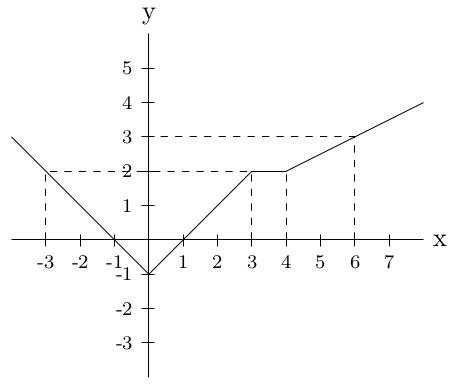
\includegraphics[width=55mm]{func1.png} \vfill
		\answer $f: \mathbb{R} \to \mathbb{R} ~|~ f(x)=\left\{\begin{matrix}-x-1 ~~~si~ x\leq0~~~~~\\~x-1 ~~~si~ 0<x\leq 3 \\ ~~2~~ ~~~~~si~ 3<x\leq4 \\ ~~\frac{1}{2}x~~ ~~~si~ 4<x~~~~~ \end{matrix}\right.$

		\item ~\\ [-12pt] 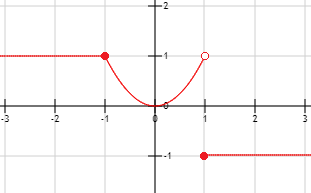
\includegraphics[width=55mm]{func2.png} \vfill
		\answer $f: \mathbb{R} \to \mathbb{R} ~|~ f(x)=\left\{\begin{matrix}~1 ~~~si~ x\leq-1~~~~~\\~~x^2 ~~~si~ -1<x< 1 \\ ~-1 ~~~si~ 1\leq x ~~~~~~~\end{matrix}\right.$

		\item ~\\ [-12pt] 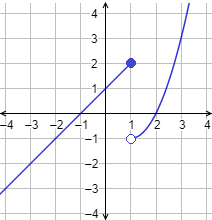
\includegraphics[width=55mm]{func3.png} \vfill
		\answer $f: \mathbb{R} \to \mathbb{R} ~|~ f(x)=\left\{\begin{matrix}~~~x+1 ~~~~~~~si~ x\leq1 \\(x-1)^2-1 ~~~si~ 1<x \end{matrix}\right.$

		\item ~\\ [-12pt] 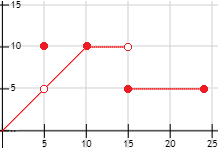
\includegraphics[width=55mm]{func4.png} \vfill
		\answer $f: [0,24] \to \mathbb{R} ~|~ f(x)=\left\{\begin{matrix}~x ~~~~ si~ x\in [0,10)\setminus\{5\}~~ \\10 ~~~~ si~ x\in\{5\}\cup[10,15) \\~5 ~~~~ si~ x\in[15,24]~~~~~~\end{matrix}\right.$

	\end{enumerate}
	\end{multicols}

	\exercise En cada caso y de ser posible, calcular las funciones $g \circ f$ y $f \circ g$:
	%\begin{multicols}{2}
	\begin{enumerate} [label=(\alph*)]
		\item $f,g:\mathbb{R} \to \mathbb{R}$ con $f(x)=3x$ ~y~ $g(x)=x-1$
		\item $f,g:\mathbb{R} \to \mathbb{R}$ con $f(x)=\lfloor x \rfloor$ ~y~ $g(x)=x^2$
		\item $f:\mathbb{R} \to \mathbb{R} ~|~ f(x)=2x$ ~y~ $g:\left[0,+\infty\right) \to \left[0,+\infty\right) ~|~ g(x)=\sqrt{x}$
		\item $f,g:\mathbb{R} \to \mathbb{R}$ con $f(x)=\sin(x)$ ~y~ $g(x)=3x+4$
		\item $f,g:\mathbb{R} \to \mathbb{R}$ con $f(x)=3x$ ~y~ $g(x)=\left\{\begin{matrix}x+3 ~~~ si ~~x\leq 6\\ x+5 ~~~ si ~~x>6\end{matrix}\right.$
		\item $f,g:\mathbb{R} \to \mathbb{R}$ con $f(x)=|x|$ ~y~ $g(x)=x+4$
		\item $f:\left(0,+\infty\right) ~|~ f(x)=\log(x)$ ~y~ $g:\mathbb{R} \to \mathbb{R} ~|~ g(x)=x^2$
		\item $f,g:\mathbb{R} \to \mathbb{R}$ con $f(x)=e^{x}$ ~y~ $g(x)=|x|$
		\item $f:\mathbb{R}\setminus\{0\} \to \mathbb{R} ~|~ f(x)=\displaystyle{\frac{1}{x}}$ ~y~ $g:\mathbb{R} \to \mathbb{R} ~|~ g(x)=\cos(x)$

	\end{enumerate}
	%\end{multicols}

	\exercise Dadas $f,g,h: \mathbb{R} \to \mathbb{R}$. Definir $f \circ g \circ h$ y $h \circ g \circ f$. 
	%\begin{multicols}{2}
	\begin{enumerate} [label=(\alph*)]
		\item $f(x)=x^2+2x$, $g(x)=\displaystyle\frac{x}{4}$ y $h(x)=x+12$.
	\end{enumerate}
	%\end{multicols}

	\exercise Considerando la función $f(x)=x^2$ y las funciones a continuación, definir las siguientes funciones componiendo $f$ con las funciones $h_1(x)=x+1$, $h_2(x)=-x$ y $h_3(x)=2x$.
	\begin{multicols}{3}
	\begin{enumerate} [label=(\alph*)]
		\item $(x+2)^2$
		\item $-x^2$
		\item $x^2+2$
		\item $2x^2$
		\item $\left(\displaystyle\frac{x}{2}\right)^2$
		\item $\displaystyle\frac{x^2}{2}$
		\item $(x-3)^2-1$
		\item $(x-1)^2-3$
		\item $(x-1)^2-1$
	\end{enumerate}
	\end{multicols}

	\exercise Considerando la función $f(x)=|x|$ y las funciones a continuación, definir las siguientes funciones componiendo $f$ con las funciones $h_1(x)=x+1$, $h_2(x)=-x$ y $h_3(x)=2x$.
	\begin{multicols}{3}
	\begin{enumerate} [label=(\alph*)]
		\item $|x|+2$
		\item $|x+1|+2$
		\item $-|x|-3$
		\item $-\displaystyle\frac{|x|}{2}$
		\item $-|x|$
		\item $-|x+1|$
		\item $2|x|$
		\item $|x|-2$
		\item $-2|x|$
		\item $|x+2|+1$
		\item $-\left|\displaystyle\frac{x}{2}\right|$
		\item $\displaystyle\frac{|x|}{2}$
	\end{enumerate}
	\end{multicols}

	\exercise Resolver las siguientes ecuaciones:
	%\begin{multicols}{2}
	\begin{enumerate} [label=(\alph*)]
		\item $2^x=10$
		\item $2\ln(x)=4$
		\item $e^{x^2+1}=\displaystyle{\frac{1}{e^2}}$
		\item $\ln(x)+\ln(x^2)=-\ln(6)$
	\end{enumerate}
	%\end{multicols}

	\exercise Graficar las siguientes funciones e indicar el dominio e imagen:
	\begin{multicols}{3}
	\begin{enumerate} [label=(\alph*)]
		\item $2\ln(x)$
		\item $\ln(x)+1$
		\item $\ln(x-4)$
		\item $-\ln(x)$
		\item $-3\ln(x+1)-2$
		\item $\ln(-x)$
		\item $\log_2(x^2)$
		\item $e^{2x}$
		\item $e^{-x}$
		\item $3e^{x}$
		\item $-e^{4x}$
		\item $e^{x-2}$
		\item $2^{x+1}$
	\end{enumerate}
	\end{multicols}

	\exercise Graficar las siguientes funciones e indicar el dominio e imagen:
	\begin{multicols}{3}
	\begin{enumerate} [label=(\alph*)]
		\item $\sin(2x)$
		\item $3\sin(x)$
		\item $-2\sin(x)$
		\item $\sin(x-\pi)$
		\item $\sin(\pi x)+5$
		\item $\sin(-x)$
		\item $-2\sin\left(x-\frac{\pi}{2}\right)+4$
		\item $2\cos(3x)$
		\item $-\cos\left(x-\frac{\pi}{2}\right)$
		\item $\cos(2x+100\pi)$
		\item $\arcsin(x)$
		\item $\arccos(x)$
		\item $\arctan(x)$
	\end{enumerate}
	\end{multicols}

	\exercise Resolver las siguientes ecuaciones hallando todas las soluciones posibles.
	\begin{multicols}{3}
	\begin{enumerate} [label=(\alph*)]
		\item $2\sin(x)=1$
		\item $3\sin(x)=0$
		\item $4\sin^{2}\left(x-\frac{\pi}{2}\right)=0$
		\item $\sin(x)-\frac{\sqrt{3}}{2}=0$
		\item $2\cos(-x)=\sqrt{2}$
		\item $20\cos(x)+60=-80$
	\end{enumerate}
	\end{multicols}

	\exercise Graficar las siguientes funciones.
	\begin{multicols}{3}
	\begin{enumerate} [label=(\alph*)]
		\item $\displaystyle\frac{2}{x}$
		\item $\displaystyle\frac{x+1}{x+1}$
		\item $\displaystyle\frac{2x+3}{4x-1}$
		\item $x^2-4x+4$
		\item $x^2-5$
		\item $-x^2+1$
		\item $3(x+1)(x-1)$
		\item $(x-1)^2-16$
		\item $4(x+1)^2-4$
		\item $\sqrt{x}$
		\item $\sqrt{-2x}$
		\item $\sqrt{x^2}$
		\item $2\sqrt{x+1}$
		\item $\sqrt{4x}+5$
		\item $-\sqrt{x}+3$
	\end{enumerate}
	\end{multicols}

	\exercise Hallar $f \circ g$ y graficarla.
	%\begin{multicols}{2}
	\begin{enumerate} [label=(\alph*)]
		\item $f(x)=\sin(x)$ ~y~ $g(x)=2x$
		\item $f(x)=\sqrt{x}$ ~y~ $g(x)=3x-1$
		\item $f(x)=\ln(x)$ ~y~ $g(x)=x-1$
		\item $f(x)=\displaystyle{e^{-x}}$ ~y~ $g(x)=\ln(x)$
		\item $f(x)=\sqrt{x}$ ~y~ $g(x)=\ln(x-1)$
		\item $f(x)=\ln(x)$ ~y~ $g(x)=x^2+4$
		\item $f(x)=\sin(x)$ ~y~ $g(x)=\displaystyle{e^{x^2-2x+1}}$
	\end{enumerate}
	%\end{multicols}

	\exercise Hallar la función inversa cuando sea posible, indicando el dominio e imagen.
	%\begin{multicols}{2}
	\begin{enumerate} [label=(\alph*)]
		\item $f(x)=\displaystyle\frac{2x-1}{3}$
		\item $g(x)=2x^2+x-1$
		\item $h(x)=\ln(x^2-1)+5$
		\item $i(t)=\displaystyle{4+16 e^{-\frac{1}{2}t}}$
	\end{enumerate}
	%\end{multicols}

\end{enumerate}

\end{document}